\documentclass[a4paper,11pt] {article}
\usepackage{graphicx}
\usepackage{amssymb, amsmath, amsthm}
\usepackage{setspace}
\usepackage{amsfonts}
\usepackage{algorithm}
\usepackage[noend]{algpseudocode}
\usepackage{multirow}% http://ctan.org/pkg/multirow
\usepackage{hhline}% http://ctan.org/pkg/hhline
%-----------Margin, Linespread, Spacing-----------%
\usepackage[letterpaper, margin=1.3in]{geometry}
\usepackage[letterpaper]{geometry}
\linespread{1}
%-------------------------------------------------%

%-----------Define header and footnotes-----------
\usepackage{fancyhdr}               % Header and footnotes
\pagestyle{fancy}
\lhead{\bfseries \scriptsize CQF}
\chead{\bfseries \scriptsize Module 3 Solution}
\rhead{\bfseries \scriptsize Ran Zhao}
\renewcommand{\headrulewidth}{0.4pt}
%-------------------------------------------------%

%---------------------Listings--------------------%
\usepackage{listings}
\usepackage{color}
\definecolor{dkgreen}{rgb}{0,0.6,0}
\definecolor{gray}{rgb}{0.5,0.5,0.5}
\definecolor{mauve}{rgb}{0.58,0,0.82}
\lstset{
  language=Octave,                % the language of the code
  basicstyle=\footnotesize,           % the size of the fonts that are used for the code
  numbers=left,                   % where to put the line-numbers
  numberstyle=\tiny\color{gray},  % the style that is used for the line-numbers
  stepnumber=2,                   % the step between two line-numbers. If it's 1, each line
                                  % will be numbered
  numbersep=5pt,                  % how far the line-numbers are from the code
  backgroundcolor=\color{white},      % choose the background color. You must add \usepackage{color}
  showspaces=false,               % show spaces adding particular underscores
  showstringspaces=false,         % underline spaces within strings
  showtabs=false,                 % show tabs within strings adding particular underscores
  frame=single,                   % adds a frame around the code
  rulecolor=\color{black},        % if not set, the frame-color may be changed on line-breaks within not-black text (e.g. commens (green here))
  tabsize=2,                      % sets default tabsize to 2 spaces
  captionpos=b,                   % sets the caption-position to bottom
  breaklines=true,                % sets automatic line breaking
  breakatwhitespace=false,        % sets if automatic breaks should only happen at whitespace
  title=\lstname,                   % show the filename of files included with \lstinputlisting;
                                  % also try caption instead of title
  keywordstyle=\color{blue},          % keyword style
  commentstyle=\color{dkgreen},       % comment style
  stringstyle=\color{mauve},         % string literal style
  escapeinside={\%*}{*)},            % if you want to add LaTeX within your code
  morekeywords={*,...}               % if you want to add more keywords to the set
}
%-------------------------------------------------%

\makeatletter
\def\BState{\State\hskip-\ALG@thistlm}
\makeatother

%----------------Title, Author, Dates-------------
\author{Ran Zhao}
\title{Asian Option Pricing using Monte Carlo Simulation}
\date{}
\begin{document}
\maketitle
%--------------------------------------------------


\section{Stock Price Simulation}
\subsection{Milstein Scheme Simulation}
The underlying stock price follows the Geometric Brownian Motion (GBM), whose dynamic is

\begin{equation} \label{eqn::GBM}
dS_t = r_t S_t dt + \sigma_t dW_t
\end{equation}
where $r_t$ is the short rate at time $t$, and $\sigma_t$ is the implied volatility at time $t$. $W_t$ is the Wiener process.

The Forward Euler-Maruyama methods for the GBM gives

$$
S_{t+\Delta t} - S_t = r_t S_t \Delta t + \sigma_t \phi \sqrt{\Delta t}
$$
where $\Delta t$ refers to as the time step in discrete time. And $\phi$ is a standard normal random number. That is, $\phi \sim N(0,1)$.

The Milstein method corrects the Forward Euler-Maruyama with a term on error level of $O(\delta t)$. Given a stochastic process $Y_t$ with

$$
dY_t = A(Y_t,t) dt + B(Y_t,t)dW_t
$$

the discretization using Milstein scheme is

$$
Y_{t+\Delta t} - Y_t = A \Delta t + B\phi \sqrt{\Delta t} + \frac{1}{2} B \frac{\partial B}{\partial Y_t} (\phi^2 - 1) \Delta t
$$
where $\frac{1}{2}(\phi^2 - 1) \Delta t$ is the Milstein correction term. For GBM, the Milstein scheme yields

$$
S_{t+\Delta t} - S_t = r_t S_t \Delta t + \sigma_t S_t \phi \sqrt{\Delta t} + \frac{1}{2} S_t \sigma^2 (\phi^2-1) \Delta t
$$

\subsection{Antithetic Variance Reduction}
The antithetic variable technique attempts to reduce the variance by introducing negatively correlated random numbers between pair of observations. While simulating the GBM, one set of standard normal random numbers is generated, labeled as $\phi^{n} \sim N(0,1)$. Then $-\phi^{n}$ also has a standard normal distribution. Regular normal random number generating methods include Box-Muller method and Polar-Marsaglia method.

The pairs $\{(\phi^{n},-\phi^{n})\}$ are distributed more desirable than $2n$ independent samples, since the samples with antithetic variable have mean 0 and negative correlation.

The whole simulation procedure is shown in Algorithm~\ref{alg:esg}.

\begin{algorithm}
\caption{Stock Price Generation}\label{alg:esg}
\begin{algorithmic}[1]
\Procedure{$S_T$ Projection}{$S_0,T-t,\sigma,r$} %\Comment{The g.c.d. of a and b}
\State $S_1(0,:) = S_0$, $S_2(0,:) = S_0$
\State $N = (T-t)/\Delta t$ \Comment{Define number of time steps}
\For{$i=1$ to $N$} %\Comment{We have the answer if r is 0}
\For{$\omega=1$ to $M$}    \Comment{Define number of scenarios}
\State Generate $\phi$
\State $S_1(i,\omega)= S_1(i-1,\omega) * (1 + r * \Delta t + \sigma * \phi * \sqrt{\Delta t} + \frac{1}{2} * \sigma^2 *(\phi^2-1)*\Delta t)$
\State $S_2(i,\omega)= S_2(i-1,\omega) * (1 + r * \Delta t + \sigma * (-\phi) * \sqrt{\Delta t} + \frac{1}{2} * \sigma^2 *(\phi^2-1)*\Delta t)$
\EndFor
\EndFor %\label{euclidendwhile}
\State \textbf{return} $\{S_1, S_2\}$  %\Comment{The gcd is b}
\EndProcedure
\end{algorithmic}
\end{algorithm}

In this report, the input parameters for the simulation are set as $S0 = 100$, $E = 100$, $T-t=1$, $\Delta t = 1/365$, $\sigma = 20\%$, $r = 5\%$ and $\omega = 1000$. Therefore, each time step represents a time increment of one calendar day, and there will be 2000 scenarios/paths of underlying stock price using antithetic variable.

\subsection{Simulation Testing}
Before being used into the Asian option pricing, the stock price simulations need to be tested to ensure their mathematical or statistical properties. The main testings focus on the normal random number generation and martingale property of the underlying stock price.

Figure~\ref{fig::esg_test} presents the main testing results on the simulated stock price dynamics. The left graph plots one particular (randomly selected) stock price path over the simulation period. The stock price is simulated using Milstein scheme, where there is a correction term on the order of $O(\Delta t)$. The middle graph testifies the distribution of the random numbers that simulate the Wiener process $W_t$. The blue mark draws the empirical QQ plot of the random numbers used in the stock price simulation, which is compared to the standard normal distribution QQ plot (red line). The blue labels are within a reasonable range around the red line, which indicates that the random numbers approximately follow the standard normal distribution.

The right graph plots the averaged discounted stock price over each simulation periods. The theoretical base of this testing is the martingale property of the risk neutral pricing, that is

$$
\mathbb{E}\left[e^{-\int_0^t r_s ds}S_t\right] = S_0
$$

Hence the expected value of the discounted stock price should be $S_0$. In the right graph of Figure~\ref{fig::esg_test}, the blue line is then (equally) averaged discounted stock price at each time period, and the red line is the reference line at $S_0$ level. The comparison graph shows that the simulated stock prices are within the range of $[99.8,100.2]$, which is $\pm 0.2$ around $S_0$. The simulations pass the martingale test.

\begin{figure}
  \centering
  %\raggedleft
  % Requires \usepackage{graphicx}
  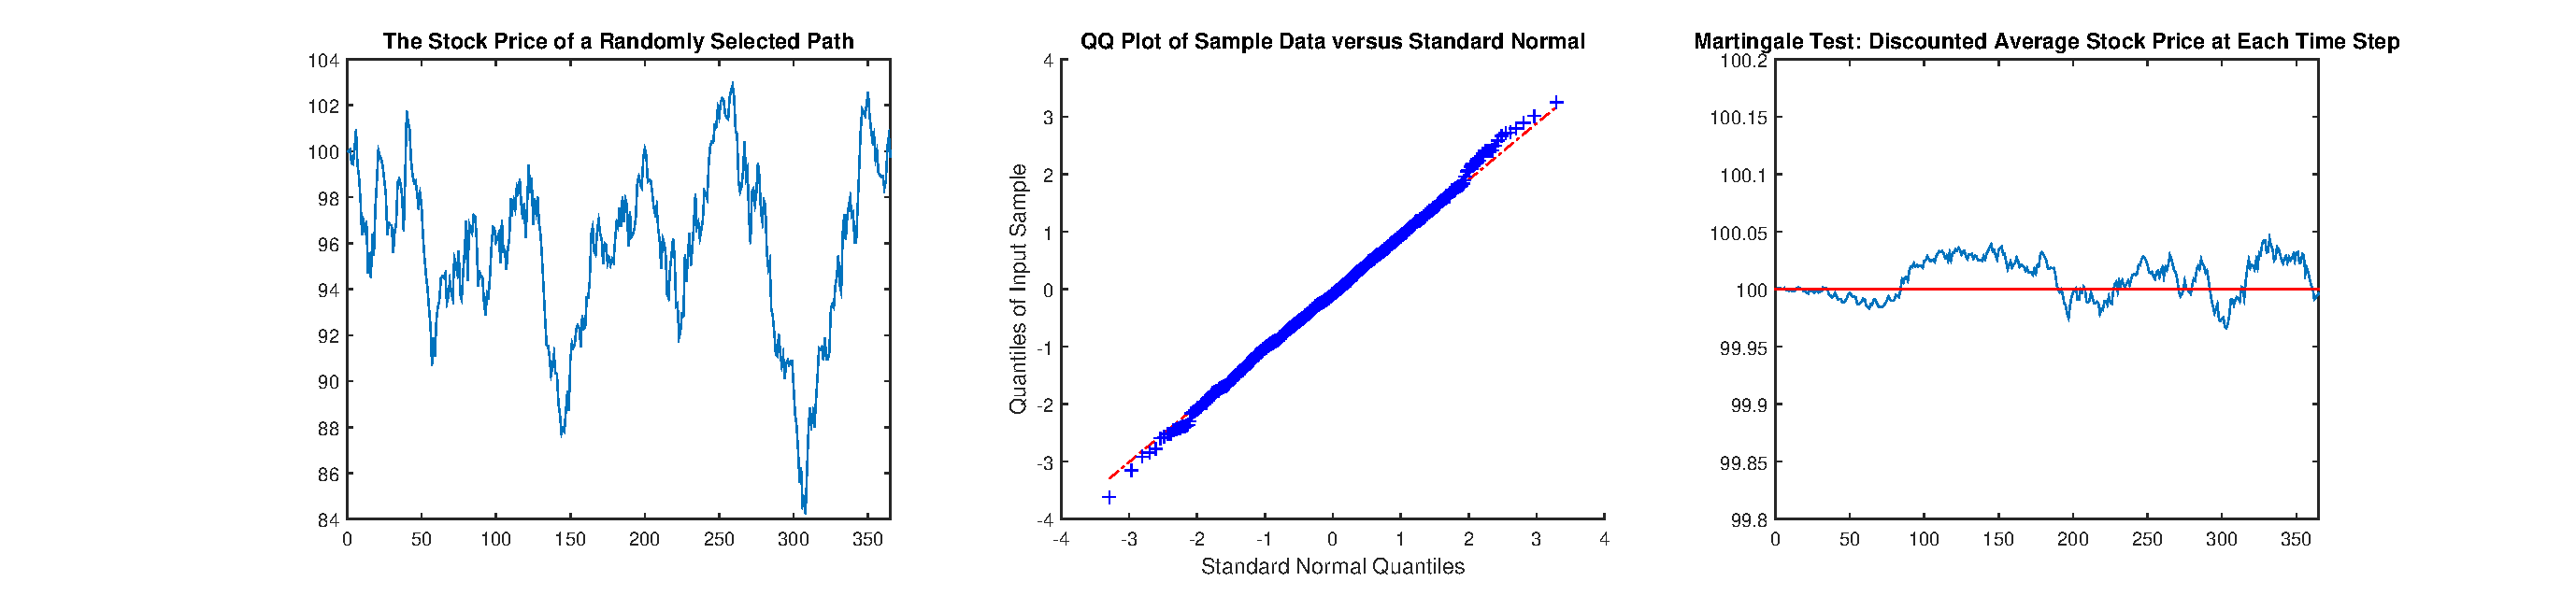
\includegraphics[scale=0.36]{esg_test.eps}\\
  \caption{The testings on the stock price simulation, including plot of a randomly selected stock price path (left), QQ plot of the random numbers for the same scenario (middle) and discounted stock price over the simulation period (right).}\label{fig::esg_test}
\end{figure}


\section{Asian Option Pricing}
\subsection{Payoff Scheme}
In general, the expected value of the discounted payoff under the risk neutral density $\mathbb{Q}$ is

$$
V(S(T),T) = \mathbb{E}^{\mathbb{Q}} \left[e^{-\int_t^T r_\tau d\tau} \textrm{\bf Payoff } (S(T)) \right]
$$

The payoff of the Asian option varies on option type (Call vs. Put), averaging method (Arithmetic vs. Geometric sampling) and strike scheme (Fixed vs. Floating strike) and so on. This report mainly discuss the option pricing differences on averaging methods and strike schemes.

\subsubsection{Averaging Method}
Consider a regular fixed strike Asian option. An Asian call option pays out
$$
C(T) = \max(A(0,T)-K,0)
$$
where $A(0,T)$ is the averaged underlying price over the period $[0,T]$.

Under arithmetic averaging scheme, the continuous time formula of the average is
$$
A(0,T) = \frac{1}{T} \int_0^T S(t)dt
$$

In discrete time, the arithmetic average is
$$
A(0,T) = \frac{1}{N+1} \sum_{i=0}^{N} S(t_i) \qquad t_i = i \cdot \frac{T}{N}
$$
Here the ending (time) point of the stock price is included into averaging calculation. Though this ending point is excluded from the averaging in some literature, the pricing impact of the exclusion will be trivial.

Under geometric averaging scheme, the continuous time formula of the average is
$$
A(0,T) = \exp\left(\frac{1}{T} \int_0^T \ln(S(t))dt\right)
$$

In discrete time, the geometric average is
$$
A(0,T) = \left( \prod_{i=0}^{N+1} S(t_i)  \right)^\frac{1}{N+1} \qquad t_i = i \cdot \frac{T}{N}
$$

For Asian put option, the payoff function is
$$
P(T) = \max(K-A(0,T),0)
$$
and the formulae for the geometric and arithmetic averaging are the same as that of the call option.

Figure~\ref{fig::geo_vs_arith} shows the stock price simulation and its arithmetic (red) and geometric (green) averages. The Asian option has the feature that its final payoff is related to these averages.

\begin{figure}
  \centering
  %\raggedleft
  % Requires \usepackage{graphicx}
  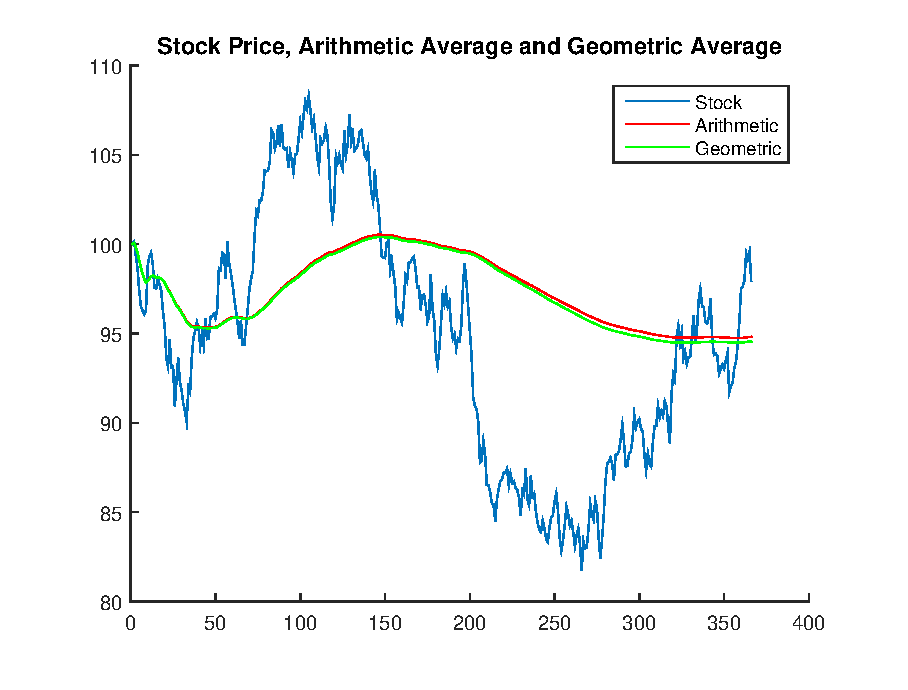
\includegraphics[scale=0.6]{geo_vs_arith.eps}\\
  \caption{The stock price dynamics and its arithmetic and geometric averages.}\label{fig::geo_vs_arith}
\end{figure}


Table~\ref{table:fixed_strike} presents the Asian option pricing results using arithmetic or geometric averaging methods. The call and put option prices with different number of paths are calculation given the simulation results. Approximately there is $\pm 0.4 \%$ difference between arithmetic and geometric results. The results are not very sensitive to the number of scenarios once it passes 10,000.

\begin{table}[htb]
\begin{center}
\begin{tabular}{c||c|c|c|c}
  \hline
  % after \\: \hline or \cline{col1-col2} \cline{col3-col4} ...
  Fixed Strike & \multicolumn{2}{c|}{Call} & \multicolumn{2}{c}{Put} \\ \hline
  Averaging & Arithmetic & Geometric & Arithmetic & Geometric \\ \hline
  1,000 & 5.6991 & 5.4916 & 3.3107 & 3.4248 \\
  10,000 & 5.7328 & 5.5181 & 3.3238 & 3.4415 \\
  100,000 & 5.7424 & 5.5262 & 3.3285 & 3.4465 \\
  \hline
\end{tabular}
\caption{The Asian pricing results on call and put option type with arithmetic or geometric averaging methods. The pricing results with 1000, 10000, 100000 paths are compared.}
\label{table:fixed_strike}
\end{center}
\end{table}


\subsubsection{Strike Scheme}
Beside the averaging method, the strike scheme also affects the payoff of the Asian option. The fixed strike Asian call option has the payoff
$$
C(T) = \max(A(0,T)-K,0)
$$

For Asian put option, the fixed strike payoff is
$$
P(T) = \max(K-A(0,T),0)
$$

And the floating strike (floating rate) Asian call option has the payoff
$$
C(T) = \max(S(T)-kA(0,T),0)
$$
where $k=1$ in this report. For Asian put option, the floating strike payoff is
$$
P(T) = \max(kA(0,T)-S(T),0)
$$

Table~\ref{table:floating_strike} presents the Asian option pricing results using arithmetic or geometric averaging methods under the floating strike scheme. The call and put option prices with different number of paths are calculation given the simulation results. Approximately there is $\pm 0.4 \%$ difference between arithmetic and geometric results. The results are not very sensitive to the number of scenarios once it passes 10,000. Comparing to the fixed strike scheme pricing, the floating strike scheme consistently has higher option price except for the Geometric averaging method of put option pricing.

\begin{table}[htb]
\begin{center}
\begin{tabular}{c||c|c|c|c}
  \hline
  % after \\: \hline or \cline{col1-col2} \cline{col3-col4} ...
  Floating Strike & \multicolumn{2}{c|}{Call} & \multicolumn{2}{c}{Put} \\ \hline
  Averaging & Arithmetic & Geometric & Arithmetic & Geometric \\ \hline
  1,000 & 5.7635 & 5.9615 & 3.3585 & 3.2349 \\
  10,000 & 5.8262 & 6.0333 & 3.3782 & 3.2528 \\
  100,000 & 5.8489 & 6.0574 & 3.395 & 3.2692 \\
  \hline
\end{tabular}
\caption{The Asian pricing results on call and put option type with arithmetic or geometric averaging methods. The pricing results with 1000, 10000, 100000 paths are compared.}
\label{table:floating_strike}
\end{center}
\end{table}

\subsection{Comparison with Theoretical Price}
Given the GBM dynamic for the underlying stock price movement and $S_{avg}$ as the geometric average of the stock price, $S_{avg}$ is also lognormally distributed. Under the risk neutral assumption, assumption, the geometric average price option can be treated like a regular option with the volatility $\sigma_{adj}$ set equal to $\sigma\sqrt{3}$ and the adjust the dividend yield equal to

$$
q_{adj} = r - \frac{1}{2} (r-q-\frac{\sigma^2}{6}) = \frac{1}{2} (r+q+\frac{\sigma^2}{6})
$$

Using the Black-Scholes-Merton formula, we price geometric average price Asian options as

\begin{eqnarray*}
C(0) &=& S_0 e^{-q_{adj}T} N(d_1) - Ke^{-rT}N(d_2) \\
P(0) &=& Ke^{-rT}N(-d_2) - S_0 e^{-q_{adj}T} N(-d_1)
\end{eqnarray*}
where
\begin{eqnarray*}
\sigma_{adj} &=& \sigma\sqrt{3} \\
q_{adj} &=& \frac{1}{2} (r+q+\frac{\sigma^2}{6}) \\
d_1 &=& \frac{1}{\sigma_{adj}\sqrt{T}}\left( \log(\frac{S_0}{K})+ (r-q_{adj}+\frac{1}{2}\sigma_{adj}^2)T\right) \\
d_2 &=& d_1 - \sigma_{adj}\sqrt{T}
\end{eqnarray*}

An arithmetic average of a set of lognormal random variables is not itself lognormal. This distribution is expressed by the German–Yor formulas. And we can approximate this complicated distribution by a lognormal distribution by using the Turnbull–Wakeman approximation.

The first moment of the continuous arithmetic average price distribution in $[t,T]$.

$$
M_1 = \frac{e^{(r-q)T}-1}{(r-q)T}S_0
$$

The second moment of the continuous arithmetic average:

$$
M2 = \frac{2e^{2(r-q)+\sigma^2}S_0^2}{(r+q+\sigma^2)(2r-2q+\sigma^2)T^2} + \frac{2S_0^2}{(r-q)T^2}\left(\frac{1}{2(r-q)+\sigma^2}-\frac{e^(r-q)T}{r-q+\sigma^2}\right)
$$

If we assume the the average asset price is lognormal, the arithmetic average price option can be treated like an option on a future contract, where:

\begin{eqnarray*}
F_0 &=& M_1 \\
\sigma_{adj}^2 &=& \frac{1}{T} \log(\frac{M_2}{M_1^2})
\end{eqnarray*}

By using the Black-Scholes-Merton formula, we price arithmetic average price Asian options:


\begin{eqnarray*}
C(0) &=& e^{-rT}(F_0 N(d_1)-KN(d_2)) \\
P(0) &=& e^{-rT}(KN(-d_2)-F_0 N(d_1))
\end{eqnarray*}
where
\begin{eqnarray*}
F_0 &=& M_1 \\
\sigma_{adj}^2 &=& \frac{1}{T} \log(\frac{M_2}{M_1^2}) \\
d_1 &=& \frac{1}{\sigma_{adj}\sqrt{T}}\left( \log(\frac{F_0}{K})+ \frac{1}{2}\sigma_{adj}^2)T\right) \\
d_2 &=& d_1 - \sigma_{adj}\sqrt{T}
\end{eqnarray*}

The comparison between the (approximate) theoretical option price and simulation option price are shown in Table~\ref{table::theo_vs_empi}. For both call option and put options, simulated price from more scenarios consistently is closer to the theoretical value, whichever averaging method is chosen (either arithmetic or geometric). Another interesting observation is that call option prices from simulations are generally more accurate than the option price simulations, in terms of the comparison to the theoretical value. A more puzzling phenomenon is that all the simulations tend to underestimate the Asian option. A plausible explanation is that the volatility term is underestimated, which causes both call and put options to be underpriced. The potential solution is to model the underlying stock price by stochastic volatility models.

\begin{table}[htb]
\begin{center}
\begin{tabular}{c||c|c|c|c|c|c|c}
  \hline
  % after \\: \hline or \cline{col1-col2} \cline{col3-col4} ...
  Type & Path/Avg. & Arith. & Theo. Arith. & \% Diff & Geo. & Theo. Geo. & \% Diff \\ \hline
\multirow{3}{*}{Call}	&	1000	&	5.6991	&	5.7828	&	-1.45\%	&	5.4916	&	5.5468	&	-1.00\%	\\
	&	10000	&	5.7328	&	5.7828	&	-0.86\%	&	5.5181	&	5.5468	&	-0.52\%	\\
	&	100000	&	5.7424	&	5.7828	&	-0.70\%	&	5.5262	&	5.5468	&	-0.37\%	\\ \hline
\multirow{3}{*}{Put}	&	1000	&	3.3107	&	3.3646	&	-1.60\%	&	3.4248	&	3.4633	&	-1.11\%	\\
	&	10000	&	3.3238	&	3.3646	&	-1.21\%	&	3.4415	&	3.4633	&	-0.63\%	\\
	&	100000	&	3.3285	&	3.3646	&	-1.07\%	&	3.4465	&	3.4633	&	-0.49\%	\\
  \hline
\end{tabular}
\caption{Comparison between Asian option simulations and theoretical values. Dimensions include option type (call or put), scenario numbers (1000, 10000 or 100000) and averaging method (arithmetic or geometric). The strike scheme is the fixed strike.}
\label{table::theo_vs_empi}
\end{center}
\end{table}


\section{Extensions}
\subsection{Stochastic Volatility Modeling}
A vast of empirical researches have shown that the implied volatilities in the real world should not assume to be constant over time and moneyness, which is opposite to model setup in the classic Black-Scholes model. In economic scenario generation, stochastic volatility models are widely used to provide market consistency stock price paths. In this report, Heston (1993) model is considered to be an extension to the regular Geometric Brownian Motion, and the corresponding Asian option pricing capability is compared to the GBM dynamic.

The Heston model specification on stock price is

$$
dS_t = \mu S_t dt + \sqrt{\nu_t} S_t d W_t^S
$$
with an additional stochastic volatility process

$$
d\nu_t = \kappa(\theta - \nu_t) dt + \xi \sqrt{\nu_t} d W_t^\nu
$$
where $d W_t^S d W_t^\nu = \rho dt$. The simulation algorithm is shown in Algorithm~\ref{alg::stochastic_vol}.

\begin{algorithm}
\caption{Stock Price Generation}\label{alg::stochastic_vol}
\begin{algorithmic}[1]
\Procedure{$S_T$ Projection Stochastic Volatility}{$S_0, \nu_0,T-t,\sigma,\kappa,\theta,\xi,\rho,r$} %\Comment{The g.c.d. of a and b}
\State $S(0,:) = S_0$
\State $N = (T-t)/\Delta t$ \Comment{Define number of time steps}
\For{$i=1$ to $N$} %\Comment{We have the answer if r is 0}
\For{$\omega=1$ to $M$}    \Comment{Define number of scenarios}
\State Generate $\phi_1$ and $\phi_2$ with correlation $\rho$
\State $\nu(i,\omega)= \nu(i-1,\omega)  + \kappa(\theta - \nu_t) \Delta t + \xi * \phi_2 * \sqrt{\nu(i-1,\omega) \Delta t} + \frac{1}{4} * \xi^2 *(\phi^2-1)*\Delta t$
\State $S(i,\omega)= S(i-1,\omega) * (1 + r * \Delta t + \sqrt{\nu(i,\omega) \Delta t} * \phi_1 + \frac{1}{2} * \nu(i,\omega) *(\phi^2-1)*\Delta t)$
\EndFor
\EndFor %\label{euclidendwhile}
\State \textbf{return} $\{S\}$  %\Comment{The gcd is b}
\EndProcedure
\end{algorithmic}
\end{algorithm}

The Asian option pricing accuracy with Heston model is not expected to over-perform the Geometric Brownian Motion process. The argument is that the Heston model has no data to calibrate in current context. However, the practical utilization will benefit from this stochastic volatility model, since it provides more market associated and consistent stock price dynamics. For illustration purpose, the Heston parameters are conjectured based on the Black-Scholes parameters given in the context, with $\kappa = 1.05, \xi = 0.35, \rho = -0.5, \nu_0 = 0.04, \theta=0.0625$. Table~\ref{table::theo_vs_empi_heston} contains the results from the Heston model simulations. The Asian option pricing results converge to the theoretical values with the increase of the number of scenarios. Though the pricing accuracy is not strictly better than the Geometric Brownian Motion, the (almost consistently) overestimation on Asian option price is mainly from the higher implied volatility target used in the Heston model (the long term volatility target is 25\%, compared to the 20\% initial value).

\begin{table}[htb]
\begin{center}
\begin{tabular}{c||c|c|c|c|c|c|c}
  \hline
  % after \\: \hline or \cline{col1-col2} \cline{col3-col4} ...
  Type & Path/Avg. & Arith. & Theo. Arith. & \% Diff & Geo. & Theo. Geo. & \% Diff \\ \hline
\multirow{3}{*}{Call}	&	1000	&	5.9547	&	5.7828	&	2.97\%	&	5.6939	&	5.5468	&	2.65\%	\\
&	10000	&	5.953	&	5.7828	&	2.94\%	&	5.6921	&	5.5468	&	2.62\%	\\
&	100000	&	5.8867	&	5.7828	&	1.80\%	&	5.6313	&	5.5468	&	1.52\%	\\ \hline
\multirow{3}{*}{Put}	&	1000	&	3.4938	&	3.3646	&	3.84\%	&	3.6428	&	3.4633	&	5.18\%	\\
&	10000	&	3.4334	&	3.3646	&	2.04\%	&	3.583	&	3.4633	&	3.46\%	\\
&	100000	&	3.3962	&	3.3646	&	0.94\%	&	3.4398	&	3.4633	&	-0.68\%	\\
  \hline
\end{tabular}
\caption{Comparison between Asian option simulations and theoretical values, using the Heston (1993) volatility model for stock price generation.}
\label{table::theo_vs_empi_heston}
\end{center}
\end{table}

\subsection{Stochastic Interest Rate Modeling}
The constant interest rate assumption can also be extended to have stochastic feature. In this report, the CIR model for spot rate is selected to price the Asian option. The CIR model specification is

$$
dr_t = (\eta-\gamma r_t) dt + \sqrt{\alpha r_t} d W_t
$$

The Milstein scheme discretized simulation will be

$$
r_{t+\Delta t} = r_t + (\eta-\gamma r_t) \Delta t + \sqrt{\alpha r_t \Delta t} \phi + \frac{1}{4} \alpha (\phi^2-1) \Delta t
$$

Built on top of the Heston volatility model, the Asian option pricing results from the CIR model is shown in Table~\ref{table::theo_vs_empi_cir}. Similar to the Heston model parameter setup, the CIR model has no instruments to calibrate to in the current context. The practical use of the stochastic interest rate model to price exotic option is wide though. The Asian option simulations are slightly better than the solely Heston model.

The CIR model parameters that populate the following estimations are $\eta = 0.05, \gamma=0.8, \alpha = 0.6, r_0 =0.05$. Currently the correlation between random numbers used in interest rate model and equity is set to 0. Another numerical extension would be joint (or hybrid) calibration between IR and equity volatility models.

\begin{table}[htb]
\begin{center}
\begin{tabular}{c||c|c|c|c|c|c|c}
  \hline
  % after \\: \hline or \cline{col1-col2} \cline{col3-col4} ...
  Type & Path/Avg. & Arith. & Theo. Arith. & \% Diff & Geo. & Theo. Geo. & \% Diff \\ \hline
\multirow{3}{*}{Call}	&	1000	&	5.9304	&	5.7828	&	2.55\%	&	5.6706	&	5.5468	&	2.23\%	\\
&	10000	&	5.9019	&	5.7828	&	2.06\%	&	5.6432	&	5.5468	&	1.74\%	\\
&	100000	&	5.8867	&	5.7828	&	1.80\%	&	5.6201	&	5.5468	&	1.32\%	\\  \hline
\multirow{3}{*}{Put}	&	1000	&	3.4795	&	3.3646	&	3.41\%	&	3.628	&	3.4633	&	4.76\%	\\
&	10000	&	3.2679	&	3.3646	&	-2.87\%	&	3.5758	&	3.4633	&	3.25\%	\\
&	100000	&	3.3962	&	3.3646	&	0.94\%	&	3.4103	&	3.4633	&	-1.53\%	\\
  \hline
\end{tabular}
\caption{Comparison between Asian option simulations and theoretical values, using the CIR interest rate model for stock price generation.}
\label{table::theo_vs_empi_cir}
\end{center}
\end{table}

\section{Conclusion}
In this report, the Milstein scheme Monte Carlo simulation technique is explored and implemented into Asian option pricing. The scenarios generated from the Geometric Brownian Motion pass the distribution and Martingale testings, showing that the stock price paths have expected mathematical properties needed in risk neutral pricing. Then these paths are used in Asian option pricing with antithetic variable technique. We discussed both averaging methods (arithmetic vs. geometric) and strike scheme (fixed strike vs. floating strike). Numerical results from Monte Carlo pricing are compared to (approximation for arithmetic averaging) theoretical Asian option values. The pricing accuracy improves with the increase on the number of scenarios. Finally the Asian option pricing framework is extended to stochastic volatility model and stochastic interest rate model. Both of the extended models benefits the economic scenario generator in terms of market consistency.


%\section*{Matlab code}
%\begin{spacing}{0.9}
%\lstinputlisting[language=Matlab]{parta.m}
%\end{spacing}

\end{document} 